\label{fundamentacao_teorica}

%%%%%%%%%%%%%%%%%%%%%%%%%%%%%%%%%%%%%%%%%%%%%%%%%%%%%%%%%%%%%%%%%%%%%%%%%%

\newcommand{\texCommand}[1]{\texttt{\textbackslash{#1}}}%

\newcommand{\exemplo}[1]{%
\vspace{\baselineskip}%
\noindent\fbox{\begin{minipage}{\textwidth}#1\end{minipage}}%
\\\vspace{\baselineskip}}%

\newcommand{\exemploVerbatim}[1]{%
\vspace{\baselineskip}%
\noindent\fbox{\begin{minipage}{\textwidth}%
#1\end{minipage}}%
\\\vspace{\baselineskip}}%

%%%%%%%%%%%%%%%%%%%%%%%%%%%%%%%%%%%%%%%%%%%%%%%%%%%%%%%%%%%%%%%%%%%%%%%%%%

Este capítulo apresenta uma breve revisão conceitual da essência do que venha ser, monitoramento e arquitetura orientada à serviços. Neste seguimento, temos as descrições dos conceitos de monitoramento de sistemas distribuídos, protocolos, ferramentas de monitoramento, agente de monitoramento, instrumentação e métricas, também sobre conceitos de \acrshort{ESB}, Erlangms, \acrshort{REST} e \acrshort{JSON}. As definições de conceitos e tecnologias estudadas são de grande ajuda tanto para o entendimento do problema quanto para execução e implementação do trabalho. Por fim são apresentados trabalhos relacionados a este tema que colaboram e orientam a pesquisa e fundamentação deste trabalho.

%%%%%%%%%%%%%%%%%%%%%%%%%%%%%%%%%%%%%%%%%%%%%%%%%%%%%%%%%%%%%%%%%%%%%%%%%%

\section{Monitoramento}

O monitoramento é forma utilizada para acompanhar ou observar o andamento de um fluxo ou processo, segundo Martino Jannuzzi \cite{de2014indicadores}, na área de tecnologia da informação é responsável por verificar e coletar informações sobre funcionamento de ativos de rede ou serviços, com propósito de apresentar informações mais resumidas e favoráveis em painéis ou sistemas para a realização de monitoramento. De acordo com Hollingsworth \cite{hollingsworth2003instrumentation} o monitoramento é necessário para uma série de fins, incluindo a verificação de status, solução de problemas, ajustes de desempenho e depuração. 

%%%%%%%%%%%%%%%%%%%%%%%%%%%%%%%%%%%%%%%%%%%%%%%%%%%%%%%%%%%%%%%%%%%%%%%%%%

\subsection{Monitoramento de Sistemas Distribuídos}

Em tecnologia da informação de monitorar ativos de rede e serviços, é acompanhar, seja pelo mau funcionamento de um ativo de rede, serviço ou por uma indisponibilidade(queda de energia ou internet). Como mencionado anteriormente o ato de acompanhar o funcionamento desses recursos propõe aos gestores desses processos encontrar uma forma mais visível e gerenciável para solucionar problemas, alertar sobre possíveis falhas ou até determinar uma situação para o retorno automático desses serviços. 

O monitoramento implantado no \acrshort{CPD} para o acompanhamento dos sistemas e serviços(\textit{web services}), desenvolvidos pela unidade de desenvolvimento \textit{software} que utiliza o barramentos de serviços Erlangms, não possui um acompanhamento específico no funcionamento de seus serviços, visto que há casos e relatos de usuários que acessam os sistemas, realizam a autenticação, clicam nos menus, mas nada aparece como resultado das pesquisas e funcionalidades dos sistemas. Por dispor de uma arquitetura orientada à serviços, a camada de apresentação funciona normalmente, mas os recursos(\textit{web services}) encontram-se indisponíveis.

Sistemas distribuídos podem ser interpretados como aplicações distintas que possuem um \textit{middleware} que realize algum tipo de conexão entre as aplicações como descrevem os autores Penteado e Treveleim \cite{penteado2012jmonitor} em seu trabalho. Esses sistemas ou aplicações podem funcionar com seus serviços de forma independente, ou dependente de outros serviços de aplicações distintas, o funcionamento desses serviços são essenciais, principalmente os que são dependentes, por esse motivo a implantação do monitoramento de sistemas distribuídos é utilizada para um melhor acompanhamento e gerenciamento das aplicações e serviços para verificar o funcionamento e disponibilidade.   

%%%%%%%%%%%%%%%%%%%%%%%%%%%%%%%%%%%%%%%%%%%%%%%%%%%%%%%%%%%%%%%%%%%%%%%%%%

\subsection{Protocolos de Monitoramento}

%%%%%%%%%%%%%%%%%%%%%%%%%%%%%%%%%%%%%%%%%%%%%%%%%%%%%%%%%%%%%%%%%%%%%%%%%%

\subsubsection{SNMP}

O Protocolo Simples de Gerenciamento de Rede (\textit{\acrlong{SNMP}}) é um protocolo da camada de aplicação responsável pela transmissão de dados e informações de gerenciamento e monitoramento entre dispositivos e ativos de rede. De acordo com Roohi \textit{et al.} \cite{roohi2014application}, o \acrshort{SNMP} é um dos protocolos mais utilizados atualmente, devido a sua arquitetura que dispõe de uma estrutura simples capaz de realizar o monitoramento em tempo real sem comprometer a eficiência que está sendo monitorado. Nesse sentido os autores Presuhn e Mankin \cite{roohi2014application,presuhn2002management} descrevem  em seu trabalho, como o \acrshort{SNMP} gerencia os ativos de rede baseando-se no esquema cliente-servidor, onde os dispositivo e ativos de rede recebem um agente para que essas informações sejam coletadas e transmitidas, por conta desse paradigma e fácil implantação a popularidade do protocolo aumentou, permitindo as empresas fornecerem diversos tipos de estruturas denominadas \acrshort{MIBs}. Os \acrshort{MIBs} são objetos criados e definidos por meio de uma estrutura virtual capaz de armazenar de informações de gerenciamento.

O autor Nadeau\cite{nadeau2003mpls} cita três componentes que formam o \acrshort{SNMP}:  

    \begin{itemize}
    \item \acrshort{SMI}
    
    Alinguagem de modelagem dos dados usados para definir \textit{syntax} dos dados de gerenciamento, como por exemplo, o tipo de objeto "INTEGER".
    
    \item \acrshort{MIBs}
    
    Estrutura usada para formar um modelo de dados do sistema(objetos), responsável por representar o tipo, definir o comportamento e a política de acesso aos objetos.
    
    \item \acrshort{SNMP}
    
    Que consiste em sua arquitetura, o gerente, um dispositivo a ser gerenciado e um agente, que dispõe das seguintes operações:
    
        \begin{itemize}
        \item GET
        
        Operação utilizada para recuperar o valor de uma instância específica de um objeto gerenciado.
        
        \item GET-NEXT
        
        Operação utilizada para percorrer interativamente o \acrshort{OID}.
        
        \item GET-BULK
        
        Operação utilizada para recuperar informações de um grupo de objetos.
        \item SET
        
        Operação utilizada para modificar o valor de uma instância de objeto.
        \item TRAP
        
        Operação utilizada para que um agente possa reportar uma notificação de forma assíncrona aos gerentes.
        
        \end{itemize}
        
    \end{itemize}
    
Após a realização de uma análise, estudos e definições, obteve-se de forma empírica o respaldo para utilização do protocolo na implementação do projeto, vale também observar que o \acrshort{CPD} utiliza o protocolo para o monitoramento de seus ativos de rede, conforme a representação na figura \ref{fun:fig:snmpexecution} apresentada a seguir.

\begin{figure}[H]
	\begin{center}
	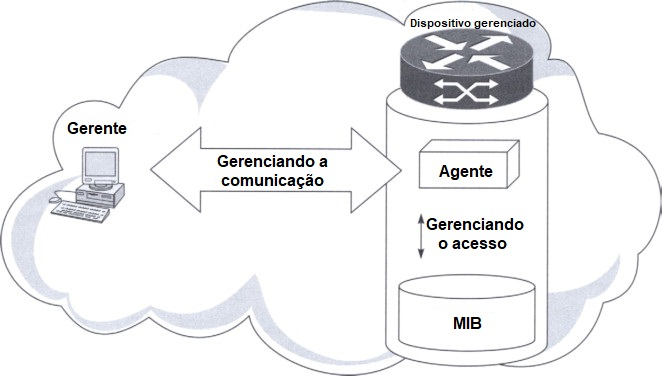
\includegraphics[scale = 0.70]{img/SNMP-Execution.jpg}
		\caption{Gerente e Agente comunicando por meio do protocolo SNMP\cite{nadeau2003mpls}}
		\label{fun:fig:snmpexecution}
	\end{center}
\end{figure}

%%%%%%%%%%%%%%%%%%%%%%%%%%%%%%%%%%%%%%%%%%%%%%%%%%%%%%%%%%%%%%%%%%%%%%%%%%

\subsubsection{GOSIP}

O \acrshort{GOSIP} é um protocolo pertencente ao modelo \acrshort{OSI} que funciona por meio de software na camada de aplicação em dispositivos \textit{peer-to-peer}, teve seu lançamento anunciado no fim da década de 80 e inicio da década de 90, para facilitar a comunicação e transferência de dados em um modelo governamental prometendo ser a comunicação integrada de sistemas militares do futuro, houve até a formalização de um documento nos padrões \acrshort{RFC} o RFC 1169, como descreve o autor Mankin\cite{mankin1991towards}, porém Harris\cite{harris1992tactical} descreve em seu trabalho que o protocolo proposto foi implementado com seus objetivos bem definidos, mas que não obtiveram o sucesso almejado, pois esperava-se que pela realização fim-a-fim conseguiriam obter melhores resultados em relação a economia da largura de banda e melhor desempenho com a redundância dos dados.

Apesar dos relatos citados no parágrafo anterior sobre as expectativas não alcançadas com o protocolo, há uma técnica bastante importante que foi extraída, e que é utilizada por meio dos dispositivos de modo a garantir que a comunicação e transmissão da informação sejam garantidas. Diante desse cenário o protocolo trabalha de forma epidêmica, disseminando facilmente as informações nos sistemas distribuídos em larga escala, cujo principal objetivo é propagar rapidamente essas informações, o que permite a realização de um monitoramento \textit{peer-to-peer},onde os dispositivos se comunicam diretamente como afirma Tanenbaum \cite{tanenbaum2007distributed}, a representação dessa propagação poderá ser visualizada na figura \ref{fun:fig:gosip}. 

\begin{figure}[H]
	\begin{center}
	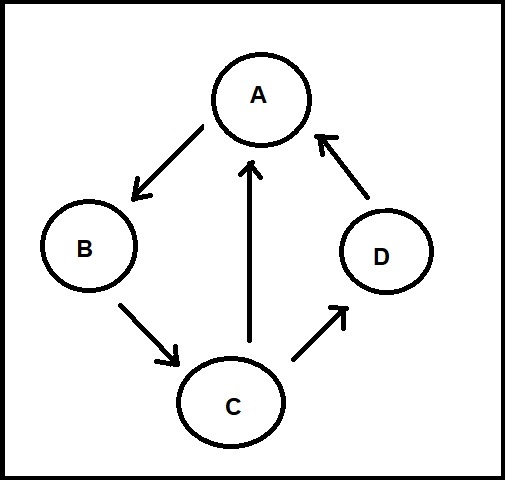
\includegraphics[scale = 0.70]{img/gosip.jpg}
		\caption{Representação de propagação epidêmica \autor{Felipe Evangelista}{dos Santos}  }
		\label{fun:fig:gosip}
	\end{center}
\end{figure}

\subsubsection{Escolha do Protocolo}

Neste trabalho, o \acrshort{GOSIP} não foi utilizado no experimento, foi utilizado como fonte de pesquisa para a realização de um comparativo conceitual e  tecnológico entre os protocolos, que permitem avaliar e auxiliar na escolha do \acrshort{SNMP} como protocolo a ser utilizado no projeto. 

%%%%%%%%%%%%%%%%%%%%%%%%%%%%%%%%%%%%%%%%%%%%%%%%%%%%%%%%%%%%%%%%%%%%%%%%%%

\subsection{Ferramentas de Monitoramento}

Na monitoração de ativos de rede ou \textit{softwares} alcançar um nível satisfatório de cobertura das aplicações é um desafio, no mercado existem diversas ferramentas relacionadas ao monitoramento. Com o aumento da disponibilidade de serviços tanto das redes como de \textit{softwares}, é quase inviável acompanhar o funcionamento sem uma ferramenta com especificidade para o monitoramento, o que subsidia necessariamente a escolha de uma solução tecnológica. Nessa seção serão apresentadas as ferramentas de monitoramento de mercado que serão examinados seus prós e contras.

\subsubsection{Nagios\textsuperscript{\textregistered}}

O Nagios\textsuperscript{\textregistered} é uma aplicação com interface \textit{web} para o monitoramento de rede baseada na web idealizada e desenvolvida por Ethan Galstad \cite{bin2011new}. O Nagios\textsuperscript{\textregistered} é projetado para a realizar o acompanhamento de ativos de rede, sistemas e serviços com a finalidade de notificar os usuários e responsáveis pelos ativos de rede, sistema e serviços que estão registrados na ferramenta como contatos emergenciais, caso aconteça alguma anomalia ou problema durante o funcionamento da rede, sistemas e serviços.

O Nagios\textsuperscript{\textregistered} é uma ferramenta que possui uma alta complexidade em sua configuração, pois possui uma gama de recursos e funcionalidades disponíveis para sua utilização, devido a grande quantidade de recursos, o Nagios\textsuperscript{\textregistered} é bastante utilizado pois também possui um grande número de \textit{plug-ins} disponíveis para realização do monitoramento, assim podendo personalizar o monitoramento de serviços como SMTP,\acrshort{SMNP}, POP3, HTTP, PING \cite{lcc2012nagios}. Nesse projeto o Nagios\textsuperscript{\textregistered} será utilizado como ferramenta de monitoramento dos sistemas e serviços fornecidos pela \acrshort{UnB} com utilização de serviço \acrshort{SMNP} para o monitoramento, haja visto que o \acrshort{CPD} já utiliza a ferramenta para o monitoramento dos ativos de rede em toda a Universidade. 

\begin{figure}[H]
	\begin{center}
	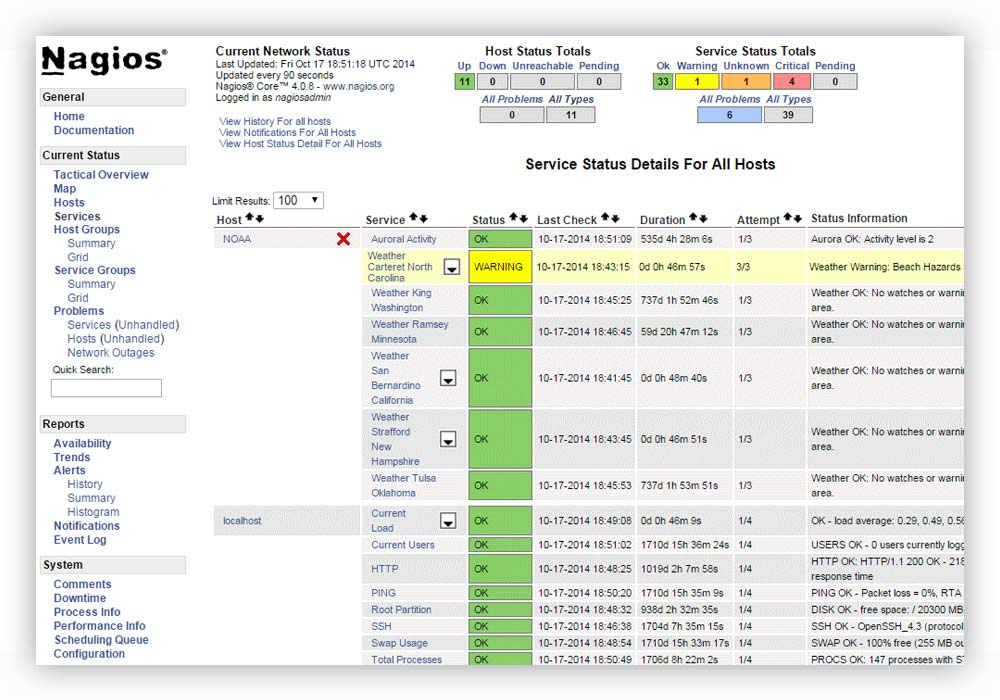
\includegraphics[scale = 0.39]{img/Comprehensive_Monitoring_Drop2.jpg}
		\caption{Monitoramento de componentes\cite{lcc2012nagios}}
		\label{fun:fig:nagios}
	\end{center}
\end{figure}

%%%%%%%%%%%%%%%%%%%%%%%%%%%%%%%%%%%%%%%%%%%%%%%%%%%%%%%%%%%%%%%%%%%%%%%%%%

\subsubsection{Ganglia}

 O Ganglia é um \textit{software} de monitoramento escalonável, com a finalidade de coletar dados para acompanhar o funcionamento de sistemas distribuídos e sistemas de alto desempenho, como \textit{clusters}. Por conta da estrutura hierárquica implementada, o \textit{software} utiliza a linguagem de marcação de texto XML para a representação dos dados. 
 
 O os autores Vyas \textit{et al.} \cite{vyas2014embedding} relatam em seu trabalho que o Ganglia é baseado em um protocolo \textit{multicast} de escuta e anúncio, e necessariamente precisa ter em cada \textit{host} que será monitorado a instalação de um \textit{Gmond}. O \textit{Gmond} é um serviço em execução em cada \textit{host} que coleta as informações de estado de um \textit{host} de forma individual e insere essas informações no canal de comunicação \textit{multicast} para enviar esse dados ao Ganglia.
 
 \begin{figure}[H]
	\begin{center}
	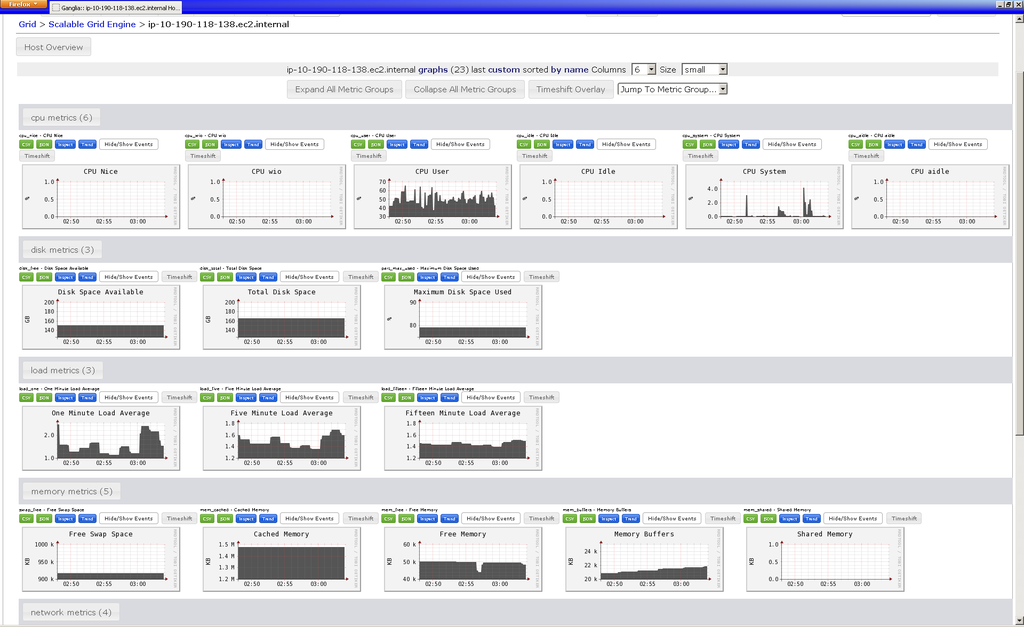
\includegraphics[scale = 0.50]{img/1024px-ScalableGridEngineGanglia2.png}
		\caption{Monitoramento de \textit{clusters} \cite{Ganglia}}
		\label{fun:fig:ganglia}
	\end{center}
\end{figure}
 
 
 Em uma breve análise após a utilização das ferramentas de monitoramento, Benincosa \cite{benincosa2ganglia} cita em seu artigo os seguintes itens:
\begin{itemize}

\item O Ganglia não possui um sistema de notificação integrado enquanto que o Nagios\textsuperscript{\textregistered} se destaca nisso.
\item Já o Nagios\textsuperscript{\textregistered} não possui agentes integrados escaláveis nos \textit{hosts} de destino (um motivo de reclamação das pessoas), enquanto que isso já faz parte do projeto original e intencional do Ganglia.

\end{itemize}

 Diante desse cenário o autor Benincosa \cite{benincosa2ganglia} sugere a utilização das ferramentas em conjunto de modo que sejam utilizados em sua potencialidade, porém como o \acrshort{CPD} já utiliza o Nagios\textsuperscript{\textregistered} e a intenção da Gestão \acrshort{CPD} e do projeto é trabalhar com o acompanhamento a notificação dos serviços caso haja alguma falha, ou mau funcionamento, e como o Ganglia não executa uma das principais funcionalidades do monitoramento, a ferramenta não entrará como \textit{software} a ser utilizado no projeto.
 
%%%%%%%%%%%%%%%%%%%%%%%%%%%%%%%%%%%%%%%%%%%%%%%%%%%%%%%%%%%%%%%%%%%%%%%%%%

\subsubsection{Cacti}

O Cacti é uma ferramenta que monitora, coleta e analisa informações por meio de gráficos em tempo de execução, com um excelente desempenho, o monitoramento pode ser feito em redes complexas e ativos de rede. O Cacti armazena suas informações coletadas em bancos de dados, para coleta das informações que são necessárias \textit{scripts}/comandos que são implementados em cada ativo e são denominados cactos, e para apresentação dos gráficos é necessário a utilização do \textit{software}  \acrfull{RRDTool}, que possui apresentação gráfica bastante intuitiva e de fácil utilização \cite{cacti}.

Segundo Oetiker\cite{rrdtool} o \acrshort{RRDTool} é uma ferramenta que realiza o registro de dados e gráficos de alto desempenho para dados de séries temporais, e como os cactos instalados nos \textit{hosts} são \textit{scripts}, o \acrshort{RRDTool} pode ser facilmente integrado com \textit{scripts} de \textit{shell}. 

\begin{figure}[H]
	\begin{center}
	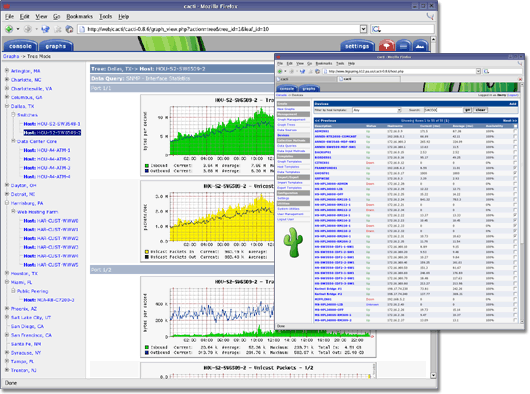
\includegraphics[scale = 0.50]{img/cacti_promo_main.png}
		\caption{Monitoramento de rede \cite{cacti}}
		\label{fun:fig:cacti}
	\end{center}
\end{figure}

O Cacti possui \textit{plugins} para integração com outras funcionalidades e ferramentas, incluído o protocolo \acrshort{SNMP}, poréma não é o seu foco devido a preocupação com o desempenho na troca de informações e no monitoramento. Como o trabalho que visa uniformizar o meio de comunicação entre as aplicações e definir especificamente um protocolo de comunicação, para transmitir informações para realização do monitoramento, esse \textit{software} não será utilizado no projeto.

\begin{figure}[H]
	\begin{center}
	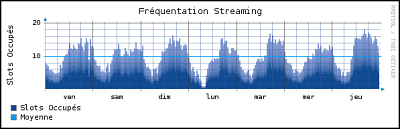
\includegraphics[scale = 0.50]{img/stream-pop.png}
		\caption{Gráfico de monitoramento do RRDTool \cite{rrdtool}}
		\label{fun:fig:rrdtool}
	\end{center}
\end{figure}

%%%%%%%%%%%%%%%%%%%%%%%%%%%%%%%%%%%%%%%%%%%%%%%%%%%%%%%%%%%%%%%%%%%%%%%%%%

\subsubsection{Zabbix}

O Zabbix é uma solução tecnológica conceituada e desenvolvida para realização de monitoramento de rede, servidores e serviços. A monitoração poderá ser realizada com o agrupamento destes recursos objetivando a potencialização das vantagens de utilização dos ativos de TI, ou a diminuição de riscos da utilização desses ativos aos usuários, esse procedimento é denominado \textit{pooling} ou por mensagens de notificações e alertas por meio de \textit{trapping}, como afirmam os autores Contessa e Fraga\cite{contessa2010gerenciamento}. O Zabbix tem como idealizador  Alexei Vladishev, e atualmente é mantido pela Zabbix SIA \cite{zabbix}.   

Como as demais aplicações e \textit{softwares} citados anteriormente, o Zabbix possui funcionalidades para monitorar e coletar de dados por servidores ou agentes, a ferramenta tem suporte ao protocolo \acrshort{SNMP} e também interface \textit{web} para visualização de gráficos gerados por meio dos dados coletados dos \textit{hosts} ou agentes. Por definição arquitetural o Zabbix é composto por componentes com funcionalidades primordiais para o seu funcionamento que são eles \cite{zabbix}: 

\begin{itemize}
\item Servidor Zabbix;
    \begin{itemize}
        \item É o componente central do Zabbix; que realiza o monitoramento ecom isso interage com os proxies e agentes, calcula as mudanças de estado nas \textit{triggers}, envia notificações, e controla o repositório central de dados.
    \end{itemize}
\item Agente Zabbix;
\begin{itemize}
        \item É o componente instalado nos servidores que monitora ativamente seus recursos e aplicações.
    \end{itemize}
\item Proxy Zabbix;
\begin{itemize}
        \item É o componente com a capacidade de realizar a coleta de dados, no lugar do Servidor Zabbix, distribuindo a carga de processamento.
    \end{itemize}
\end{itemize}

Em comparação com ferramentas mais utilizadas atualmente, os autores Marik e Ondrej \cite{marik2014comparative} descrevem em seu artigo que o Zabbix está entre as melhores aplicações, citadas neste trabalho, por possuir pré-requisitos básicos na instalação e configuração, excelente tempo de resposta em caso da falha de serviços e recursos de \acrshort{TI}, e notificações por e-mail e \acrshort{SMS}, porém o \textit{dashboard} para realização do monitoramento é complexo, e não intuitivo ao usuário, como pode ser visualizado a seguir na figura \ref{fun:fig:zabbix}, podendo não auxiliar em um gerenciamento adequado aos serviços e aplicações que são monitoradas, apesar de uma boa aplicação de monitorização, o Zabbix não será utilizado como ferramenta para este trabalho.    

\begin{figure}[H]
	\begin{center}
	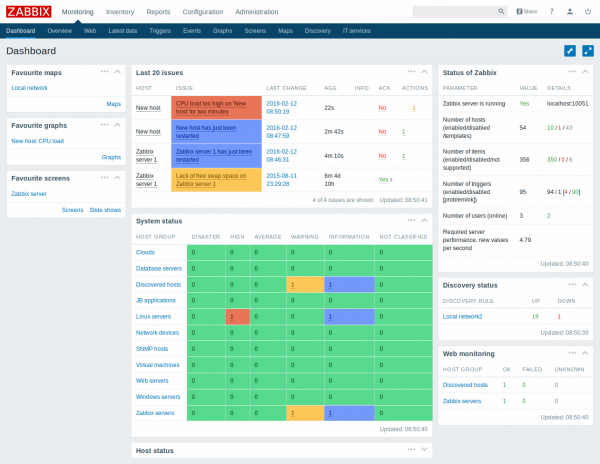
\includegraphics[scale = 0.80]{img/dashboard.png}
		\caption{\textit{Dashboard} de monitoramento \cite{zabbix}.}
		\label{fun:fig:zabbix}
	\end{center}
\end{figure}

%%%%%%%%%%%%%%%%%%%%%%%%%%%%%%%%%%%%%%%%%%%%%%%%%%%%%%%%%%%%%%%%%%%%%%%%%%

\subsection{Agente de Monitoramento}

Em uma arquitetura de monitoramento de serviços ou ativos de rede, que utilize protocolos para comunicação e transferência de dados, é necessário a implementação de agentes de monitoramento para instalação em \textit{hosts} e dispositivos, que serão monitorados, estes agentes consistem em coletar dados e enviar mensagens de alerta ao gerentes de monitoramento, como  apresentado na figura \ref{fun:fig:agente}, como por exemplo, o uso de \acrshort{CPU} e a quantidade de memória de utilização, de um processo ou um alerta de falha, de um dispositivo ou serviço, como descrevem em seu trabalho os autores Grover e Naik \cite{7439952}.  

\begin{figure}[H]
	\begin{center}
	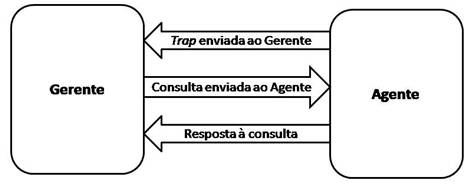
\includegraphics[scale = 0.80]{img/image004.jpg}
		\caption{Esquema de comunicação entre os agentes e as estações de gerenciamento \cite{snmpagentimage}.}
		\label{fun:fig:agente}
	\end{center}
\end{figure}

 Segundo Kazaz \textit{et al.}  \cite{6240708} um agente de monitoramento pode ser definido como um componente ou aplicação de gerenciamento de rede ou serviço no dispositivo a ser gerenciado e possuem duas operações básicas \textit{GET} e \textit{SET}, o agente em execução fica responsável por exportar os dados de gerenciamento dos sistemas, serviços ou ativos de rede gerenciados com variáveis organizadas de forma hierárquica. Essa hierarquia é contemplada por metadados que são representados por \acrshort{MIBs}, que são um conjunto de objetos gerenciados, que procuram abranger todas informações necessárias para gerência de rede. Neste trabalho o agente de monitoramento utilizado é o Exometer que funciona como agente de monitoramento responsável pela coleta das informações geradas pelo Barramento de serviços Erlangms, e a transmissão dessas informações ao Nagios\textsuperscript{\textregistered} por meio do protocolo \acrshort{SNMP}. 

%%%%%%%%%%%%%%%%%%%%%%%%%%%%%%%%%%%%%%%%%%%%%%%%%%%%%%%%%%%%%%%%%%%%%%%%%%

\subsubsection{Exometer}

\begin{figure}[H]
	\begin{center}
	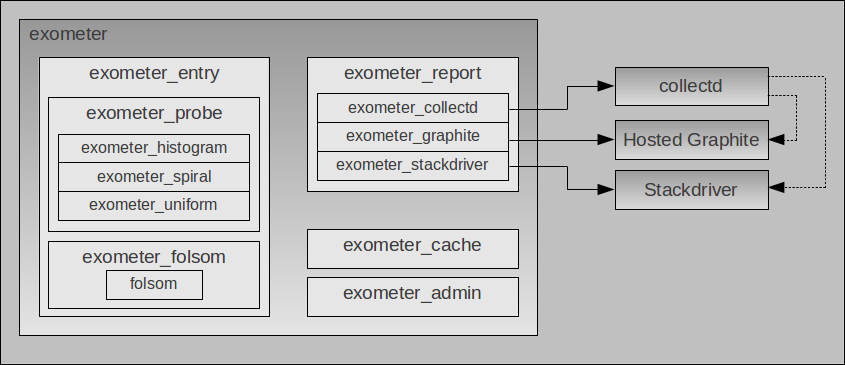
\includegraphics[scale = 0.60]{img/exometer_overview.png}
		\caption{Arquitetura do Exometer \cite{exometer_core}.}
		\label{fun:fig:zabbix}
	\end{center}
\end{figure}
O Exometer é um \textit{framework} capaz de executar a instrumentação, e permitir a exportação de dados de maneira fácil e eficiente utilizando bibliotecas implementadas em código Erlang, normalmente os dados exportados são relacionados ao desempenho dos sistemas e serviços. Com a utilização de módulos, o Exometer pode realizar a integração com uma grande variedade de sistemas de monitoramento, neste trabalho a integração é com aplicação de monitoramento Nagios\textsuperscript{\textregistered}. De acordo com Wiger \cite{exometer_core}, o potencial do Exometer é fornecer métricas de várias formas e parâmetros, para isso dispõe de um conjunto de componentes pré-definidos, que podem ser estendidos de forma personalizada para lidar com diversos tipos de métricas e alguns protocolos.

%%%%%%%%%%%%%%%%%%%%%%%%%%%%%%%%%%%%%%%%%%%%%%%%%%%%%%%%%%%%%%%%%%%%%%%%%%

\subsection{Instrumentação}
\label{instrumentacao}
Segundo Ribeiro \cite{ribeiro1999instrumentaccao} a instrumentação é uma das técnicas que utiliza instrumentos para a medição e monitoração. A instrumentação é muito utilizada no ambiente industrial, principalmente no que tange a medição dos equipamentos de produção que necessitam de acompanhamento para verificação de pressão, temperatura, vazão e nível. Os instrumentos podem estar associados e
aplicados à alguns equipamentos, como por exemplo, forno, refrigerador,
aquecedor, condicionador de ar e compressor. A operação da instrumentação funciona para que possam ser observados os instrumentos para a medição, alarme e monitoração. De acordo com Robinson \cite{robinson2002monitoring}, a instrumentação pode permitir que as informações criadas por meio da execução de instrumentos(código-fonte de \textit{software}) possam ser interferidas no funcionamento das aplicações.

O barramento de serviços Erlangms dispõe em sua arquitetura uma estrutura facilitada para sua instrumentação, e ainda possui um modelo de dados em que são registrados contadores. No modelo de dados são registradas algumas informações como; a data e hora do registro, o identificador do contador e a descrição do contador.  
Segundo os autores Frota e Finkelstein \cite{frota2008educaccao} a instrumentação pode ser utilizada como um componente de processamento da informação de sistemas de medição. Por isso a instrumentação pode ser considerada não apenas como ferramenta de contagem de valores para medição, e poderá ser utilizada também como uma forma de aprendizagem conceitual e científica.  

%%%%%%%%%%%%%%%%%%%%%%%%%%%%%%%%%%%%%%%%%%%%%%%%%%%%%%%%%%%%%%%%%%%%%%%%%%

\subsection{Métricas de Monitoramento}

A métrica de \textit{software} é uma das opções que possibilita acompanhar o funcionamento das aplicações por meio de dados e registros, como afirmam os autores Castro e Hernandes \cite{de2016metrica}. À medida que os sistemas e serviços crescem em quantidade, tamanho, complexidade e criticidade, a necessidade de monitorá-los é cada vez mais evidente. 

Nesse seguimento os autores Munawar, Jiang, Reidemeister e Ward  \cite{5298441}, descrevem que o monitoramento representa o acompanhamento dessas aplicações de forma detalhada e clara aos responsáveis pelas aplicações. A ISO/IEC 9126-1 \cite{associaccao2003nbr} descreve e normatiza a forma para medir a qualidade de \textit{software}, de acordo com a norma \cite{associaccao2003nbr}, a métrica é o método e escala de medição definidos, a métrica pode ser direta ou indireta, a medição de uma métrica direta se dá quando não depende de medidas de outros atributos e a métrica indireta se dá quando há ou existe a necessidade de derivação de um ou mais atributos de medição.

No que tange um ambiente computacional, as métricas ajudam a medir o \textit{software} de uma forma eficaz, para isso é preciso que as métricas sejam bem definidas, justificadas e formalizadas, além disso é desejável que as métricas apresentem de forma clara o que está sendo medido, descrevam rapidamente a medição sem custeio computacional alto e que o resultado do que está sendo medido não seja mudado ou sofra interferência em seu resultado caso haja a mudança de \textit{software}, plataforma ou linguagem de programação, conforme Meirelles \cite{meirelles2013monitoramento} relata em sua tese.

%%%%%%%%%%%%%%%%%%%%%%%%%%%%%%%%%%%%%%%%%%%%%%%%%%%%%%%%%%%%%%%%%%%%%%%%%%

\section{Arquitetura Orientada a Serviços - SOA}

A Arquitetura Orientada a Serviços é um estilo arquitetural que permite realizar a comunicação entre aplicações heterogêneas por meio de mensagens, como afirmam os autores Fraser, Rankine e Woodcock\cite{fraser2007service}. Na implementação e disponibilização de \textit{softwares}, comum que essas aplicações possuam estruturas e linguagens completamente distintas, pois essas aplicações independem umas das outras, mas precisam que a comunicação entre elas aconteça. Para que haja a comunicação interoperável entre as aplicações é previsto na arquitetura \acrshort{SOA} que serviços(\textit{web services}) possam ser utilizados como componentes distribuídos, que ao mesmo tempo que possam fornecer informações, mas possam também consumi-las, conforme descrição dos trabalho dos autores Sward,  Boleng e Bianco \textit{et al.}: \cite{sward2011service,bianco2011architecting}.

O Manifesto \acrshort{SOA} apresenta uma proposta de definição da conceituação para área. A partir do manifesto as discussões não cravam apenas conceitos, criavam orientações para guiar as organizações de maneira consistente e sustentável, de modo a agregar valor ao negócio, com maior agilidade e efetividade de custos, em alinhamento com a dinâmica das necessidades de negócio,priorizando os seguintes itens, como afirmam os autores Erl \textit{et al.} \cite{erl2009soa}.

\begin{itemize}

\item Valor do negócio em relação a estratégia técnica;

\item Objetivos estratégicos em relação a benefícios específicos de projetos;

\item Interoperabilidade intrínseca em relação a integração personalizada;

\item Serviços compartilhados em relação a implementações de propósito específico;

\item Flexibilidade em relação a otimização; e

\item Refinamento evolutivo em relação a busca da perfeição inicial.

\end{itemize}

Para realização da comunicação entre as aplicações ou serviços em componentes distribuídos no estilo arquitetural \acrshort{SOA}, os autores Clements \textit{et al.}  \cite{clements2002documenting} descrevem em seu trabalho que a comunicação poderá ser executada por meio de um intermediador ou na falta dele poderá ser realizada ponto-a-ponto. Entre os intermediadores do estilo arquitetural \acrshort{SOA}, os autores Bass \textit{et al.} \cite{bass2003software} citam que a arquitetura dispõe dos seguintes tipos de componentes que compõem uma arquitetura orientada a serviços, são eles :

\begin{itemize}

\item Prestador de serviços;

\item Consumidores de serviço;

\item \acrfull{ESB};

\item Registro de serviços;

\item \textit{Server Orchestration}; 

\item \acrfull{SOAP}.

\item \acrfull{REST}

\item Conector de mensagens assíncronas

\end{itemize}

Com a utilização desses componentes, os autores Bass \textit{et al.}  \cite{bass2003software} tratam como principal benefício de uma arquitetura \acrshort{SOA} a interoperabilidade, pois permite que aplicações, dispositivos, sistemas e serviços heterogêneos possam realizar a comunicação entre si, fornecendo e consumindo informações  de forma integrada. 

O \acrshort{CPD} para implementação e implantação da arquitetura \acrshort{SOA} na modernização dos seus sistemas, escolheu como componente o \acrshort{ESB} e como plataforma o barramento Erlangms\cite{Agilar},que atua como intermediador prestando serviço de mensageria.

%%%%%%%%%%%%%%%%%%%%%%%%%%%%%%%%%%%%%%%%%%%%%%%%%%%%%%%%%%%%%%%%%%%%%%%%%%

\subsection{\textit{Enterprise Service Bus} - ESB}

Um componente \acrshort{ESB} é fornece o serviço de infraestrutura e intermedeia a comunicação por meio de serviços entre aplicações consumidoras e fornecedoras de serviços, fazendo de forma uniforme a transmissão das mensagens por meio de um protocolo ou tecnologia, utilizando conectores do tipo \textit{Call-return}, onde os mais comuns e também mais utilizados no mercado são o \acrshort{SOAP} e o \acrshort{REST}, como descrevem  os autores Clements \textit{et al.} \cite{clements2002documenting}.

Para a implementação de um \acrshort{ESB} no estilo \acrshort{SOA} a organização ou instituição deverá avaliar as tecnologias utilizadas em seus sistemas ou serviços, visto que, a complexidade de uma arquitetura \acrshort{SOA} é alta, segundo os autores Bianco \textit{et al.} \cite{bianco2011architecting}, dependendo da situação não é necessário a implementação ou implantação de um \acrshort{ESB} quando por exemplo, uma organização que  possui em sua arquitetura de sistemas a mesma linguagem, plataforma e tecnologia, podendo fazer a comunicação ou troca de mensagens ponto-a-ponto. Nesse seguimento os autores Bianco \textit{et al.} \cite{bianco2011architecting} descrevem sobre o caso em que existe a necessidade da implementação ou implantação de um \acrshort{ESB}, a padronização e táticas descritas no trabalhos dos autores Bianco \textit{et al.}  \cite{bianco2011architecting} e que devem ser seguidas, e de acordo com manifesto \acrshort{SOA}\cite{erl2009soa} e possuem as seguintes características:

\begin{itemize}

\item Roteamento Intermediário - Um serviço de roteamento genérico intercepta mensagens e com base no encaminhamento a lógica que determina para onde as mensagens devem ser enviadas.

\begin{itemize}

\item Balanceamento de carga - Possuir um \textit{Failover} para um \textit{backup} no caso de o serviço de destino 	primário não estar disponível.

\item{Seleção da versão do Serviço - Verificar se os pedidos são enviados para versões compatíveis de um serviço para     suportar compatibilidade com versões anteriores durante os períodos de transição}.

\item Serviço de seleção com base em dados da mensagem - Verificar se pedidos de clientes são enviados para um componente de processamento mais rápido.

\item Regras de controle de acesso - Analisar um pedido de um usuário não autenticado é encaminhado para um início de sessão página.

\item Tratamento de exceções - Apresentar uma mensagem de erro de resposta que é redirecionada para um serviço responsável para manipulação de exceção centralizada.

\end{itemize}

\item O \textit{Service Broker} - Integrar componentes que foram desenvolvidos em diferentes linguagem por diferentes organizações.

\begin{itemize}

\item Modelo de Transformação de Dados - Os dados enviados do consumidor de serviços numa dada estrutura transforma-se em uma estrutura diferente, que está prevista para o prestador de serviços.

\item Conversão de Formato de dados - Usar sempre consumidor de serviço e o fornecedor precisa de trocar dados representados em diferentes formatos como por exemplo, \acrshort{XML}, \acrshort{CSV}, \acrshort{JSON}.

\item Protocolo \textit{Bridging} - O consumidor de serviço envia uma solicitação usando um protocolo e o \textit{Service Broker} intercepta o pedido e o converte para um pedido ao fornecedor do serviço usando um protocolo diferente.

\end{itemize}

\item Mensagens \textit{Asynchronous} - Alguns \acrshort{ESB}s fornecem capacidade suficiente, para que o sistema de mensagens permita que os pedidos e respostas de um serviço possam ser trocados através de canais de mensagens.

\item Interceptor - Alguns \acrshort{ESB}s oferecem a capacidade de configurar interceptores, que são elementos de software que são ativados para todas as solicitações e respostas.

\end{itemize}

Segundo os autores Bianco \textit{et al.} \cite{bianco2011architecting} o \acrshort{ESB} deve ter as vantagens e benefícios que uma arquitetura \acrshort{SOA} pode fornecer,  e para alcançá-los cita os seguintes itens(Atributos de Qualidade), como representação de um \acrshort{ESB} padrão e operável. O atendimento à esses itens são de suma importância:

\begin{itemize}

\item Interoperabilidade - O \acrshort{ESB} permite que sistemas diferentes possam interoperar, por meio de protocolos de comunicação, e tecnologias de implementação. 

\item Modificabilidade - A capacidade de executar a transformação do modelo de dados que permite a implantação de novas versões de um serviço, sem interromper consumidores de serviços existentes. 

\item Confiabilidade - Quando o receptor de uma solicitação de serviço ou resposta falhou, e o ESB cria ou gera uma fila, para que a mensagem seja executada para quando o serviço estiver disponível novamente. 

\item Segurança - O \acrshort{ESB} pode incluir a funcionalidade do controle de acesso. Pode aplicar a autenticação e regras de autorização em trocas de mensagens de serviço.

\end{itemize}

O \acrshort{ESB} deve responder a altura seus \textit{trade-offs},  principalmente em uma arquitetura complexa como esta, entre os desafios que deverão ser suportados, para um bom funcionamento da plataforma, os autores Bianco \textit{et al.} \cite{bianco2011architecting} citam:

\begin{itemize}

\item Manutenibilidade - Ter cuidado e atenção ao especificar demais a codificação do \acrshort{ESB}, ao ponto de restringir comunicação com outras tecnologias. 
 	
\item Performance - Não permitir a perda comprometedora no desempenho do \acrshort{ESB}, por conta das lógicas de roteamento ou interpretação dos dados durante a comunicação.

\item Segurança - verificar a configuração a fim de evitar acessos não autorizados ao \acrshort{ESB}.

\item Disponibilidade - O \acrshort{ESB} pode ser um ponto único de falha no sistema.

\end{itemize}

%%%%%%%%%%%%%%%%%%%%%%%%%%%%%%%%%%%%%%%%%%%%%%%%%%%%%%%%%%%%%%%%%%%%%%%%%%

\subsection{Erlangms}
O Barramento de serviços da \acrshort{UnB} denominado Erlangms foi conceituado em uma disciplina do \acrshort{MPCA}, e proposto como trabalho para solucionar alguns problemas relacionados a quantidade de sistemas heterogêneos, defasagem tecnológica das aplicações e a falta de um padrão de comunicação entre eles no \acrshort{CPD}, como Agilar \cite{Agilar} descreve em seu trabalho. 

O Erlangms dispõe de uma arquitetura \acrshort{SOA}, com o estilo arquitetural \acrshort{REST} e sua implementação foi feita na linguagem funcional Erlang. O barramento atualmente está implantado no \acrshort{CPD}, e  funcionando com um serviço de mensageria. A realização da comunicação e troca de mensagens dos sistemas e clientes, é feita por meio de serviços(\textit{web services}) utilizando o formato \acrshort{JSON}. O modelo arquitetural do Erlangms é apresentado na figura \ref{fun:fig:Erlangms} .

\begin{figure}[H]
	\begin{center}
	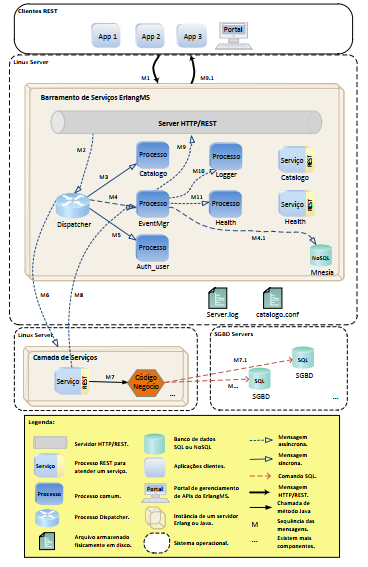
\includegraphics[scale = 1.30]{img/Arquitetura_ErlangMS.png}
		\caption{Arquitetura do trabalho Erlangms descrita por\cite{Agilar}}
		\label{fun:fig:Erlangms}
	\end{center}
\end{figure}

%%%%%%%%%%%%%%%%%%%%%%%%%%%%%%%%%%%%%%%%%%%%%%%%%%%%%%%%%%%%%%%%%%%%%%%%%%

\subsection{\textit{Representational State Transfer} - REST}

A Transferência de Estado Representacional - \acrshort{REST} pode ser definida como um estilo arquitetural híbrido derivado de vários estilos arquiteturais, que são baseados em redes e que definem um conjunto de restrições e propriedades baseados no protocolo de comunicação \acrshort{HTTP}, com a intenção de fornecer a interoperabilidade entre sistemas, serviços e aplicações distribuídas e conectadas à rede mundial de computadores - \acrshort{WWW} para a realização de troca de informações, conforme descrevem os autores Fielding e Taylor \cite{fielding2000architectural}. Os \textit{web services} compatíveis com \acrshort{REST} permitem que os sistemas solicitantes acessem e manipulem representações textuais de recursos da \textit{Web} utilizando um conjunto uniforme e predefinido de operações sem estado. De acordo com os autores Booth \textit{et al.} \cite{booth2013web} o estilo arquitetural proposto por Fielding e Taylor, que inspirou a criação do documento de arquitetura definido pelo \acrshort{TAG} - \acrshort{W3C},  quanto muitos outros arquitetos de \textit{software}, que o veem como um modelo norteador para construir e padronizar serviços da Web. O \acrshort{REST} fornece semântica para uniformizar sua interface, principalmente no que tange à operações para criar, recuperar, atualizar e excluir dados, e  também a possibilidade da utilização de padrões de tecnologia como \acrshort{XML} e o \acrshort{JSON}. 

Em \acrshort{REST} as principais operações por meio do protocolo \acrshort{HTTP} são:

\begin{itemize}

\item POST - Cria uma nova entidade ou recurso. 

\item GET - Recupera a informação de um recurso.

\item PUT - Atualiza os dados de um recurso informado.

\item DELETE - Exclui os dados de um recurso informado.

\end{itemize}

%%%%%%%%%%%%%%%%%%%%%%%%%%%%%%%%%%%%%%%%%%%%%%%%%%%%%%%%%%%%%%%%%%%%%%%%%%

\subsection{\textit{JavaScript Object Notation} - JSON}

Segundo Bray \cite{bray2017javascript}, \acrfull{JSON} é um formato baseado em texto, de fácil leitura e interpretação para humanos, para a leitura de máquinas o \acrshort{JSON} é baseado em um subconjunto da linguagem de programação \textit{JavaScript}, e por possuir um um padrão, seu funcionamento independe de uma tecnologia ou linguagem de programação, focando princialmente na troca de dados e mensagens.

Por decisão técnica especificamente relacionada a interoperabilidade e o baixo acoplamento o barramento utilizado pelo \acrshort{CPD} o Erlangms, utiliza o \acrshort{JSON} por conta do  baixo \textit{overhead} gerado na troca de mensagens, em relação às trocas de mensagens feitas com a utilização protocolo \acrshort{SOAP} com a linguagem \acrshort{WSDL}, e apontando também o nível baixo da curva de aprendizagem para utilização do \acrshort{JSON}.

%%%%%%%%%%%%%%%%%%%%%%%%%%%%%%%%%%%%%%%%%%%%%%%%%%%%%%%%%%%%%%%%%%%%%%%%%%

\section{Trabalhos Relacionados}

O Abdu \textit{et al.} \cite{abdu1996monitoring} descrevem em seu trabalho sobre a opção por investigar a necessidade para realizar o monitoramento de sistemas distribuídos e a necessidade de minimizar a degradação do desempenho de sistemas monitorados. E relatam que a configuração adotada depende da informação a ser monitorada através de diretivas monitoramento.

Seguindo a preocupação com a escalabilidade do monitoramento durante o funcionamento das aplicações Repantis \textit{et al.} \cite{repantis2010scaling} cita sobre a rede Akamai, que permite o processamento dos dados de mais de 60.000 servidores de borda, em quase tempo real. A disponibilidade de uma poderosa interface SQL-like para que os dados, tem sido um elemento importante na forma como gerimos a nossa rede. Neste trabalho, têm-se centrado sobre as escolhas do design que permite a consulta para escalar conforme o tamanho da rede, o volume de dados, e o número de consultas a crescer. E mostram como a consulta aborda esses desafios de escalabilidade, ao fornecer uma latência de dados na ordem de minutos e um tempo médio de resposta de consulta na ordem de décimos de segundo.

O trabalho de Subramanyan \textit{et al.} \cite{subramanyan2000scalable} apresenta estudos sobre o atraso na execução na tarefa de monitoramento devido ao gargalo gerado durante as operações dos agentes, e também descrevem que a solução proposta e implementada utiliza o protocolo do monitoramento rede \acrshort{SNMP}, que garante uma facilidade de execução, interoperabilidade e aceitabilidade, e baseia-se nos mais recentes padrões propostas pela RFC 2592.  

Phan \cite{phan2009cryptanalysis} relata em seu trabalho sobre o nível de segurança do protocolo e questiona sobre a falta de confidencialidade e privacidade, itens faltantes no SNMPv1 e, e descreve em seu trabalho, e dispõe de um experimento, e recomenda a utilização do SNMPv3.

Com a realização da análise qualitativa, os autores Lee, Shyan e Lo Hsu \cite{lee2004design} buscaram apresentar o funcionamento do protocolo SNMP por meio de experimentos valendo-se de suas vantagens, entre elas seus principais componentes a utilização entre eles: 1) Da estação de gestão; 2) Agente de gestão; 3) Base de informações de gestão; e 4) protocolo de gestão. Eles descrevem o trabalho científico de forma conectada, concisa e objetiva, sobre as técnicas utilizadas para realização do estudo. O trabalho apresenta uma abordagem orientada à objetos, utilizada para alcançar o projeto sistemático para implementação de agentes SNMP em sistemas de monitoramento, para o gerenciamento remoto.

Em seu texto Pătruţ, Bogdan e Tomozei \cite{puatruct2010agent} expõe os resultados obtidos no desenvolvimento e manutenção de aplicações distribuídas, e sistemas de monitoramento multiagente, com exemplos práticos, a fim de implementar e testar as abordagens teóricas. Os sistemas de monitoramento de agentes múltiplos trazem qualidade e eficiência em quase todas as áreas de atividade, na qual inclui pesquisa científica, educação, saúde ou defesa.
Utilizando os conceitos sólidos da inteligência artificial e reunindo-os para os recursos infinitos dos sistemas distribuídos e da Internet, dessa forma buscando reduzir a duração do alcance dos objetivos.

Com a leitura e entendimento dos trabalhos pode-se perceber uma preocupação com a utilização do monitoramento, em relação ao desempenho, mesmo quando utilizadas técnicas e tecnologias distintas, mas observa-se a importância da realização do monitoramento, visto a grande demanda de \textit{softwares} disseminados na rede mundial de computadores.

%%%%%%%%%%%%%%%%%%%%%%%%%%%%%%%%%%%%%%%%%%%%%%%%%%%%%%%%%%%%%%%%%%%%%%%%%%%%%%%%

\section{Síntese do Capítulo}

Neste capítulo foram apresentados conceitos sobre o monitoramento de sistemas distribuídos, desde os conceitos básicos sobre monitoramento, descrevendo e conceituando sobre os protocolos disponíveis para execução do monitoramento, bem como as ferramentas que utilizam desses protocolos para realização da comunicação. Foram abordados também conceitos sobre agentes de monitoramento, técnica  de instrumentação e métricas de monitoramento e como elas funcionam, assim como o conceito arquitetural \acrshort{SOA}, e seus componentes, entre eles o barramentos de serviços utilizado pela \acrshort{UnB}. O Capítulo 3 seguinte apresenta a realização do mapeamento sistemático.

%%%%%%%%%%%%%%%%%%%%%%%%%%%%%%%%%%%%%%%%%%%%%%%%%%%%%%%%%%%%%%%%%%%%%%%%%%%%%%%%
